\documentclass[12pt,a4paper]{article}

% ── Packages ──────────────────────────────────────────────────────────────────
\usepackage[utf8]{inputenc}
\usepackage[T1]{fontenc}
\usepackage{amsmath,amssymb,amsfonts}
\usepackage{graphicx}
\usepackage{booktabs}
\usepackage{natbib}
\usepackage{hyperref}
\usepackage{geometry}
\usepackage{float}
\usepackage{caption}
\usepackage{subcaption}
\usepackage{xcolor}
\usepackage{lineno}
\usepackage{setspace}
\usepackage{enumitem}
\usepackage{multirow}

\geometry{margin=2.5cm}
\hypersetup{colorlinks=true,linkcolor=blue,citecolor=blue,urlcolor=blue}
\linenumbers
\doublespacing

% ── Title ─────────────────────────────────────────────────────────────────────
\title{A Compact Rank-1 Quadratic Approximation for Ocean Total Dissolved Inorganic Carbon Identified by Symbolic Regression}

\author{
[Author 1]$^{1}$\thanks{Correspondence: [email@institution.edu]}, [Author 2]$^{2}$, [Author 3]$^{1}$\\
\small $^{1}$[Department, University, City, Country]\\
\small $^{2}$[Institute, City, Country]
}

\date{}

\begin{document}

\maketitle

% ══════════════════════════════════════════════════════════════════════════════
% ABSTRACT
% ══════════════════════════════════════════════════════════════════════════════
\begin{abstract}
Symbolic regression was used to search for compact analytical expressions relating total dissolved inorganic carbon (TCO$_2$) to salinity ($S$), temperature ($T$), and apparent oxygen utilisation (AOU) in the global ocean. Within a restricted search space of addition, subtraction, multiplication, and division operators, PySR identified a squared-linear functional form:
\begin{equation*}
\text{TCO}_2 = (\alpha S + \beta T + \gamma \cdot \text{AOU}/100 + \delta)^2 + \epsilon\,,
\end{equation*}
which imposes a rank-1 quadratic structure---a one-dimensional nonlinear curve embedded in three-dimensional predictor space. The model was fitted per basin by nonlinear least squares to GLODAP v2.2023 data ($N = 472{,}154$ quality-controlled observations across four basins).

Validation used a chronological holdout: training on pre-2015 data, model selection on 2015--2018 data, and post-2018 observations as a temporal holdout. In the Atlantic, the quadratic model achieved $R^2 = 0.907$, RMSE $= 20.17$~$\mu$mol~kg$^{-1}$, a 13.8\% improvement over a full second-order polynomial regression benchmark (10 free parameters). In the Indian, Pacific, and Southern Ocean basins, the quadratic model (5 parameters) showed per-sample absolute errors formally equivalent to the benchmark within $\delta = 2$~$\mu$mol~kg$^{-1}$ (TOST, $p < 0.001$ in all basins), demonstrating comparable predictive accuracy with half the parameters.

Performance is strongly domain-dependent. The Atlantic shows the largest improvement, particularly at the surface (0--100~m, +23.2\%) and abyssal depths ($>$3000~m, +10.1\%). Surface predictions are less reliable ($R^2 \approx 0.76$ in the Atlantic). The Southern Ocean below 3000~m shows poor performance when the global model is applied ($R^2 = -0.174$), though a locally fitted model achieves $R^2 = 0.786$, indicating that the failure reflects inadequate generalization of global coefficients rather than inherent unpredictability.

The squared-linear structure is qualitatively consistent with nonlinear carbonate buffering, but carbonate chemistry does not uniquely imply this functional form. The result demonstrates discovery within a restricted symbolic search space, not unrestricted discovery of a fundamental ocean carbon law.
\end{abstract}

\medskip
\noindent\textbf{Keywords:} total dissolved inorganic carbon; symbolic regression; ocean carbon system; Revelle factor; GLODAP; rank-1 approximation

% ══════════════════════════════════════════════════════════════════════════════
% 1. INTRODUCTION
% ══════════════════════════════════════════════════════════════════════════════
\section{Introduction}
\label{sec:intro}

Total dissolved inorganic carbon (TCO$_2$) governs the ocean's capacity to absorb atmospheric CO$_2$ and is central to marine carbon-cycle calculations \citep{Sarmiento2006}. Empirical estimation of TCO$_2$ from more routinely measured hydrographic variables is essential for gap-filling observational datasets, quality control, and computing basin-scale carbon inventories \citep{Takahashi1993, Key2004}.

Multiple linear regression has been the standard approach for decades \citep{Goyet1991, Millero1998}, typically using salinity, temperature, and nutrients as predictors. More recent machine-learning methods---including neural networks, random forests, and gradient boosting---have achieved higher accuracy by exploiting complex nonlinear relationships \citep{Broullon2019, Carter2018}, but sacrifice interpretability: the functional form relating predictors to TCO$_2$ remains opaque.

Symbolic regression offers a different approach: searching for compact mathematical expressions that balance predictive accuracy with structural simplicity. Unlike black-box methods, the output is an interpretable equation whose form can be examined for physical consistency. Recent algorithmic advances, particularly PySR \citep{Cranmer2023}, have made it feasible to search large hypothesis spaces of candidate equations using evolutionary optimization.

Here we apply PySR to search for compact expressions relating TCO$_2$ to salinity, temperature, and apparent oxygen utilisation (AOU) across four ocean basins. We emphasize at the outset several important scoping decisions:

\begin{enumerate}[nosep]
    \item The search was restricted to the operators $+$, $-$, $\times$, $\div$, $\exp$, and $\log$. Squared-linear structures are particularly accessible to this operator set through repeated multiplication, so the result represents discovery \emph{within the chosen hypothesis space}, not unrestricted discovery of the globally optimal symbolic equation.
    \item Validation is chronological (temporal holdout), not spatially independent, because GLODAP contains repeated hydrographic sections and geographically clustered observations.
    \item The physical interpretation of the discovered structure is post-hoc and qualitative, not derived from first principles.
\end{enumerate}

The key contributions are: (1)~identification of a compact five-parameter squared-linear structure that achieves competitive accuracy; (2)~formal demonstration via TOST equivalence testing that the five-parameter model is statistically indistinguishable from a ten-parameter polynomial benchmark in per-sample predictive accuracy; (3)~systematic characterization of domain-dependent performance by basin, depth, and water mass; and (4)~honest identification of failure regimes.

% ══════════════════════════════════════════════════════════════════════════════
% 2. DATA
% ══════════════════════════════════════════════════════════════════════════════
\section{Data}
\label{sec:data}

\subsection{GLODAP v2.2023}

We used the Global Ocean Data Analysis Project version 2.2023 \citep{Lauvset2023}, extracting the following variables: salinity (\texttt{G2salinity}), temperature (\texttt{G2temperature}), apparent oxygen utilisation (\texttt{G2aou}), total dissolved inorganic carbon (\texttt{G2tco2}), latitude (\texttt{G2latitude}), longitude (\texttt{G2longitude}), depth (\texttt{G2depth}), year (\texttt{G2year}), and ocean region code (\texttt{G2region}).

\subsection{Quality Control}

Observations were retained when all of the following conditions were simultaneously satisfied:
\begin{itemize}[nosep]
    \item All variables finite
    \item $25 < S < 42$
    \item $-2.5 < T < 35$~$^\circ$C
    \item $1700 < \text{TCO}_2 < 2600$~$\mu$mol~kg$^{-1}$
    \item $\text{AOU} > -50$~$\mu$mol~kg$^{-1}$
\end{itemize}
After quality control, $472{,}154$ observations remained.

\subsection{Basin Definitions}

Four basins were defined using GLODAP region codes and latitude thresholds:
\begin{itemize}[nosep]
    \item \textbf{Atlantic}: region code 1, latitude $> 35^\circ$S
    \item \textbf{Indian}: region code 16, latitude $> 35^\circ$S
    \item \textbf{Pacific}: region code 8, latitude $> 35^\circ$S
    \item \textbf{Southern Ocean}: latitude $< 35^\circ$S, all region codes
\end{itemize}
These definitions are mutually exclusive by construction (verified: zero pairwise overlap). Table~\ref{tab:sample_sizes} reports per-basin sample sizes. Table~\ref{tab:predictor_stats} summarises predictor distributions.

\begin{table}[htbp]
\centering
\caption{Sample sizes by basin and temporal split. Training: pre-2015; test: 2015--2018; external holdout: post-2018.}
\label{tab:sample_sizes}
\begin{tabular}{lrrrr}
\toprule
\textbf{Basin} & \textbf{Total} & \textbf{Train} & \textbf{Test} & \textbf{External} \\
\midrule
Atlantic        & 147{,}387 & 125{,}701 & 11{,}436 & 10{,}250 \\
Indian          &  40{,}163 &  32{,}270 &  3{,}764 &  4{,}129 \\
Pacific         & 187{,}356 & 138{,}139 & 31{,}767 & 17{,}450 \\
Southern Ocean  &  97{,}248 &  82{,}045 &  6{,}483 &  8{,}720 \\
\midrule
\textbf{Total}  & \textbf{472{,}154} & \textbf{378{,}155} & \textbf{53{,}450} & \textbf{40{,}549} \\
\bottomrule
\end{tabular}
\end{table}

\begin{table}[htbp]
\centering
\caption{Predictor summary statistics by basin (mean $\pm$ SD).}
\label{tab:predictor_stats}
\begin{tabular}{lrrrrr}
\toprule
\textbf{Basin} & $S$ & $T$ ($^\circ$C) & AOU ($\mu$mol~kg$^{-1}$) & TCO$_2$ ($\mu$mol~kg$^{-1}$) & Depth (m) \\
\midrule
Atlantic       & $35.16 \pm 0.83$ & $8.4 \pm 6.9$  & $59 \pm 50$  & $2152 \pm 55$  & $1238 \pm 1345$ \\
Indian         & $34.96 \pm 0.64$ & $9.7 \pm 8.3$  & $133 \pm 82$ & $2201 \pm 115$ & $1358 \pm 1390$ \\
Pacific        & $34.46 \pm 0.66$ & $8.3 \pm 8.1$  & $147 \pm 101$& $2212 \pm 139$ & $1287 \pm 1470$ \\
Southern Ocean & $34.51 \pm 0.33$ & $2.3 \pm 3.8$  & $95 \pm 55$  & $2213 \pm 60$  & $1243 \pm 1364$ \\
\bottomrule
\end{tabular}
\end{table}

\subsection{Temporal Split}

The data were split chronologically:
\begin{itemize}[nosep]
    \item \textbf{Training}: pre-2015 (years 1972--2014)
    \item \textbf{Test}: 2015--2018
    \item \textbf{External holdout}: post-2018 (2018--2021)
\end{itemize}
The external holdout spans approximately 3~years with a 4-year gap from the last training observation. This is a \emph{temporal} holdout, not a spatially independent sample: GLODAP contains repeated hydrographic sections, so the holdout likely includes observations at locations similar to training data. The validation therefore tests temporal generalization within the GLODAP sampling framework, not global spatial extrapolation.

% ══════════════════════════════════════════════════════════════════════════════
% 3. METHODS
% ══════════════════════════════════════════════════════════════════════════════
\section{Methods}
\label{sec:methods}

\subsection{Symbolic Regression Configuration}
\label{sec:sr_config}

PySR \citep{Cranmer2023} was used to search for compact analytical expressions. The search configuration was:

\begin{table}[htbp]
\centering
\caption{PySR search configuration.}
\label{tab:pysr_config}
\begin{tabular}{ll}
\toprule
\textbf{Parameter} & \textbf{Value} \\
\midrule
Binary operators  & $+$, $-$, $\times$, $\div$ \\
Unary operators   & $\exp$, $\log$ \\
Predictors        & $S$, $T$, AOU/100 \\
Target            & TCO$_2$ \\
Maximum complexity & 20 \\
Populations       & 15 \\
Population size   & 50 \\
Iterations        & 50 \\
Random seed       & 42 \\
Loss function     & Mean squared error \\
Model selection   & Best (complexity--accuracy tradeoff) \\
\bottomrule
\end{tabular}
\end{table}

\textbf{Search-space limitation.} The restricted operator set makes squared-linear structures particularly accessible through repeated multiplication ($x \times x = x^2$). The discovered form therefore represents the best compact expression found within this hypothesis space, not the globally optimal symbolic equation over all possible operators. We assess robustness to this choice in Section~\ref{sec:robustness}.

\subsection{Discovered Equation}

The symbolic regression identified the following functional form, consistent across four independently fitted basins:
\begin{equation}
\text{TCO}_2 = (\alpha S + \beta T + \gamma \cdot \text{AOU}/100 + \delta)^2 + \epsilon
\label{eq:model}
\end{equation}
where $\alpha$, $\beta$, $\gamma$, $\delta$, and $\epsilon$ are fitted coefficients. This equation imposes a \textbf{rank-1 quadratic structure}: defining the core variable $z = \alpha S + \beta T + \gamma \cdot \text{AOU}/100 + \delta$, the model is $\text{TCO}_2 = z^2 + \epsilon$, which is a one-dimensional nonlinear curve embedded in three-dimensional predictor space.

\subsection{Model Fitting}

Equation~\eqref{eq:model} was fitted per basin by nonlinear least squares using the Levenberg--Marquardt algorithm (\texttt{scipy.optimize.curve\_fit}, \texttt{scipy} v1.18; Python 3.14). Initial parameter guesses were $[1.0, -0.3, 2.5, 20.0, 2000.0]$ with maximum function evaluations of 30{,}000. Table~\ref{tab:coefficients} reports the fitted coefficients.

\begin{table}[htbp]
\centering
\caption{Fitted coefficients for Equation~\eqref{eq:model}. $\sigma_{\text{resid}}$: training residual standard deviation.}
\label{tab:coefficients}
\begin{tabular}{lrrrrrr}
\toprule
\textbf{Basin} & $\alpha$ & $\beta$ & $\gamma$ & $\delta$ & $\epsilon$ & $\sigma_{\text{resid}}$ \\
\midrule
Atlantic        & 1.4859 & $-0.2377$ & 2.2196 & $-36.62$ & 1923.5 & 15.70 \\
Indian          & 0.4992 & $-0.1693$ & 1.2860 &  10.07  & 1433.1 & 16.51 \\
Pacific         & 1.1594 & $-0.2696$ & 1.7753 & $-20.15$ & 1790.3 & 15.96 \\
Southern Ocean  & 0.7289 & $-0.2307$ & 1.6378 &  $-6.20$ & 1811.2 &  9.04 \\
\bottomrule
\end{tabular}
\end{table}

\subsection{Polynomial Benchmark}

The benchmark is a full second-order polynomial regression (``MLR+AOU'') with all main effects, quadratic terms, and pairwise interactions:
\begin{equation}
\text{TCO}_2 = \beta_0 + \beta_1 S + \beta_2 T + \beta_3 A + \beta_4 S^2 + \beta_5 T^2 + \beta_6 A^2 + \beta_7 ST + \beta_8 SA + \beta_9 TA
\label{eq:mlr}
\end{equation}
where $A = \text{AOU}$. This uses \textbf{10 free parameters} (9 features + intercept) versus 5 for the quadratic model, and includes the same predictors, providing a fair comparison that controls for information content.

\subsection{Prediction Intervals}

Nominal 95\% prediction intervals were constructed via hybrid bootstrap ($n = 1{,}000$ replicates):
\begin{enumerate}[nosep]
    \item Resample training observations with replacement;
    \item Refit Equation~\eqref{eq:model} on the resampled data;
    \item Generate predictions on the test set;
    \item Add a random draw from $\mathcal{N}(0, \hat{\sigma}_{\text{resid}})$ to each prediction.
\end{enumerate}
The 2.5th and 97.5th percentiles of the resulting prediction distribution form the reported intervals. This procedure is a \emph{hybrid} bootstrap: nonparametric case resampling combined with parametric residual augmentation. It is not a purely parametric bootstrap.

\textbf{Limitation.} Observation-level resampling does not account for spatial, cruise, temporal, or depth dependence in GLODAP. We therefore also performed cluster bootstrap resampling by $5^\circ$ latitude $\times$ $10^\circ$ longitude bins (Section~\ref{sec:pi_results}).

\subsection{Hessian and Rank-1 Geometry}

For $f(\mathbf{x}) = (\mathbf{v}^T\mathbf{x} + \delta)^2 + \epsilon$ with $\mathbf{v} = (\alpha, \beta, \gamma/100)^T$, the Hessian is:
\begin{equation}
\mathbf{H} = 2\mathbf{v}\mathbf{v}^T
\label{eq:hessian}
\end{equation}
This matrix has rank~1, with sole non-zero eigenvalue $2\|\mathbf{v}\|^2$ along direction $\mathbf{v}$. The quadratic surface therefore has curvature along only one direction in predictor space, confirming the rank-1 structure.

\subsection{Robustness Testing}
\label{sec:robustness}

The stability of the discovered form was assessed through four analyses:

\begin{enumerate}[nosep]
    \item \textbf{Subsample stability}: random subsets of 30--90\% of training data (5 trials per fraction);
    \item \textbf{Random-seed sensitivity}: 8 different seeds for train/test splits;
    \item \textbf{Alternative AOU scaling}: AOU/10 versus AOU/100;
    \item \textbf{Complexity comparison}: BIC against a cubic extension with cross-terms.
\end{enumerate}
These tests assess whether the same structural family remains competitive under perturbation, not whether it is globally optimal over all possible symbolic expressions.

\subsection{Equivalence Testing}

To formally assess whether the quadratic model and polynomial benchmark have practically equivalent predictive accuracy, we applied Two One-Sided Tests \citep[TOST;][]{Schuirmann1987} on \emph{per-sample paired absolute-error differences}:
\begin{equation}
d_i = |\text{TCO}_{2,i}^{\text{obs}} - \hat{\text{TCO}}_{2,i}^{\text{MLR}}| - |\text{TCO}_{2,i}^{\text{obs}} - \hat{\text{TCO}}_{2,i}^{\text{Quad}}|
\label{eq:tost_diff}
\end{equation}
Positive $d_i$ indicates the quadratic model is more accurate for observation~$i$. The hypotheses are:
\begin{align}
H_0&: |\bar{d}| \geq \delta & \text{(not equivalent)} \label{eq:tost_h0}\\
H_1&: |\bar{d}| < \delta & \text{(equivalent)} \label{eq:tost_h1}
\end{align}
Equivalence requires both one-sided $t$-tests to reject at $\alpha = 0.05$, which is equivalent to the $100(1-2\alpha)\%$ confidence interval for $\bar{d}$ lying entirely within $[-\delta, +\delta]$. We tested with $\delta = 2$ and 5~$\mu$mol~kg$^{-1}$.

\subsection{Water-Mass Classification}

Observations were classified into water masses using temperature, salinity, depth, and latitude thresholds consistent with oceanographic conventions \citep{Tomczak2002}:
\begin{itemize}[nosep]
    \item \textbf{Surface}: depth $< 200$~m
    \item \textbf{Thermocline}: $200 < \text{depth} < 800$~m, $T > 8^\circ$C
    \item \textbf{AAIW}: $1 < T < 8^\circ$C, $33.5 < S < 34.6$, $300 < \text{depth} < 1500$~m, lat $< -15^\circ$
    \item \textbf{NADW}: $1 < T < 5^\circ$C, $34.8 < S < 35.1$, $1000 < \text{depth} < 4000$~m
    \item \textbf{AABW}: $T < 1^\circ$C, $34.6 < S < 34.75$, depth $> 3000$~m
\end{itemize}
These threshold-based definitions are approximate; density-based classification would be more rigorous but requires additional data not consistently available in GLODAP.

% ══════════════════════════════════════════════════════════════════════════════
% 4. RESULTS
% ══════════════════════════════════════════════════════════════════════════════
\section{Results}
\label{sec:results}

\subsection{Rank-1 Quadratic Structure}

The core variable $z = \alpha S + \beta T + \gamma \cdot \text{AOU}/100 + \delta$ is strongly correlated with observed TCO$_2$ (Pearson $r > 0.96$ in all basins), confirming that the model captures the dominant mode of TCO$_2$ variability through a single nonlinear dimension.

\textbf{Figure~\ref{fig:rank1} specification.} Plot TCO$_2$ versus $z$ for each basin. The data should collapse onto a single parabolic curve $z^2 + \epsilon$, demonstrating the rank-1 structure. Use density visualization for the large sample sizes.

\subsection{Temporal Validation}

Table~\ref{tab:validation} reports test-set and external-holdout metrics. The Atlantic shows the largest improvement over the polynomial benchmark (+13.8\%); the Indian, Pacific, and Southern Ocean show small differences in the opposite direction.

\begin{table}[htbp]
\centering
\caption{Test-set and external-holdout validation metrics. RMSE in $\mu$mol~kg$^{-1}$. Improvement: positive = quadratic model has lower RMSE than polynomial benchmark.}
\label{tab:validation}
\begin{tabular}{l rrrr r rrr}
\toprule
 & \multicolumn{4}{c}{\textbf{Test set (2015--2018)}} & & \multicolumn{2}{c}{\textbf{External (post-2018)}} \\
\cmidrule(lr){2-5} \cmidrule(lr){7-8}
\textbf{Basin} & $n$ & $R^2$ & RMSE & MAE & \textbf{Improv.} & $R^2$ & RMSE \\
\midrule
Atlantic        & 11{,}436 & 0.907 & 20.17 & 14.93 & $+13.8\%$ & 0.921 & 17.68 \\
Indian          &  3{,}764 & 0.985 & 14.49 & 11.06 & $-5.6\%$  & 0.968 & 18.44 \\
Pacific         & 31{,}767 & 0.985 & 16.00 & 11.09 & $-3.2\%$  & 0.990 & 13.82 \\
Southern Ocean  &  6{,}483 & 0.968 & 10.58 &  7.55 & $-1.1\%$  & 0.965 &  8.99 \\
\bottomrule
\end{tabular}
\end{table}

The polynomial benchmark has $R^2$ values of 0.875 (Atlantic), 0.987 (Indian), 0.986 (Pacific), and 0.969 (Southern Ocean), with RMSE values of 23.41, 13.73, 15.50, and 10.46~$\mu$mol~kg$^{-1}$, respectively.

\textbf{Figure~\ref{fig:scatter} specification.} Four-panel hexbin plot of observed versus predicted TCO$_2$ per basin, with 1:1 line, $R^2$, RMSE, and $n$ annotated.

\subsection{Equivalence Testing}

Table~\ref{tab:tost} reports the TOST results on per-sample paired absolute-error differences (Equation~\ref{eq:tost_diff}). All four basins achieve formal equivalence at both $\delta = 2$ and 5~$\mu$mol~kg$^{-1}$: the 95\% confidence intervals for the mean paired difference lie entirely within the equivalence bounds.

\begin{table}[htbp]
\centering
\caption{TOST equivalence test results on per-sample paired absolute-error differences (Equation~\ref{eq:tost_diff}). Positive $\bar{d}$ = quadratic more accurate. CI: 95\% confidence interval. Equivalence requires CI $\subset [-\delta, +\delta]$.}
\label{tab:tost}
\begin{tabular}{lr@{}l r@{}l rr l}
\toprule
 & \multicolumn{2}{c}{$\delta = 2$} & \multicolumn{2}{c}{$\delta = 5$} & & & \\
\cmidrule(lr){2-3} \cmidrule(lr){4-5}
\textbf{Basin} & \multicolumn{2}{c}{CI for $\bar{d}$} & \multicolumn{2}{c}{CI for $\bar{d}$} & $\bar{d}$ & $n$ & \textbf{Result} \\
\midrule
Atlantic        & $[+0.44,$ & $+0.84]$ & $[+0.44,$ & $+0.84]$ & $+0.64$ & 11{,}436 & Equiv.\ ($p < 0.001$) \\
Indian          & $[-0.60,$ & $-0.14]$ & $[-0.60,$ & $-0.14]$ & $-0.37$ &  3{,}764 & Equiv.\ ($p < 0.001$) \\
Pacific         & $[-0.43,$ & $-0.34]$ & $[-0.43,$ & $-0.34]$ & $-0.39$ & 31{,}767 & Equiv.\ ($p < 0.001$) \\
Southern Ocean  & $[+0.02,$ & $+0.09]$ & $[+0.02,$ & $+0.09]$ & $+0.05$ &  6{,}483 & Equiv.\ ($p < 0.001$) \\
\bottomrule
\end{tabular}
\end{table}

\textbf{Interpretation.} The five-parameter quadratic model is statistically indistinguishable from the ten-parameter polynomial benchmark in per-sample predictive accuracy across all basins. In the Atlantic, the quadratic model is slightly more accurate on average ($\bar{d} = +0.64$~$\mu$mol~kg$^{-1}$); in the Indian and Pacific, the benchmark is slightly more accurate ($\bar{d} = -0.37$ and $-0.39$). All differences are well within 1~$\mu$mol~kg$^{-1}$.

This result establishes \emph{practical similarity}, not \emph{superiority}: the compact model matches the benchmark's accuracy with half the parameters, but does not universally outperform it.

\subsection{Depth-Stratified Performance}

Table~\ref{tab:depth} reports depth-stratified metrics. Performance varies strongly with depth and basin.

\begin{table}[htbp]
\centering
\caption{Depth-stratified test-set performance. RMSE in $\mu$mol~kg$^{-1}$. Improvement: positive = quadratic better than polynomial benchmark.}
\label{tab:depth}
\small
\begin{tabular}{ll r rrr r}
\toprule
\textbf{Basin} & \textbf{Depth} & $n$ & $R^2$ & RMSE & Bench.\ RMSE & \textbf{Improv.} \\
\midrule
Atlantic & 0--100 m      & 3{,}469  & 0.758 & 28.01 & 36.46 & $+23.2\%$ \\
Atlantic & 100--500 m    & 2{,}477  & 0.781 & 18.23 & 16.55 & $-10.1\%$ \\
Atlantic & 500--1000 m   & 1{,}559  & 0.500 & 17.62 & 14.98 & $-17.7\%$ \\
Atlantic & 1000--3000 m  & 2{,}625  & 0.721 & 12.30 & 11.39 & $-8.0\%$ \\
Atlantic & 3000--7000 m  & 1{,}306  & 0.784 & 13.26 & 14.74 & $+10.1\%$ \\
\midrule
Indian & 500--1000 m    & 591    & 0.987 & 5.70  & 8.66  & $+34.1\%$ \\
Indian & 3000--7000 m   & 527    & 0.468 & 12.56 & 10.41 & $-20.7\%$ \\
\midrule
Pacific & 1000--3000 m  & 8{,}121 & 0.962 & 8.68  & 8.75  & $+0.8\%$ \\
\midrule
Southern Ocean & 500--1000 m   & 975    & 0.980 & 5.99  & 7.00  & $+14.4\%$ \\
Southern Ocean & 3000--7000 m  & 855    & $-0.174$ & 7.45 & 7.02 & $-6.1\%$ \\
\bottomrule
\end{tabular}
\par\medskip
\footnotesize{Selected rows shown; full table in Supplementary Material.}
\end{table}

\textbf{Key observations:}
\begin{itemize}[nosep]
    \item \textbf{Atlantic surface}: The quadratic model's strongest advantage (+23.2\%), likely reflecting nonlinear solubility and biological productivity effects.
    \item \textbf{Atlantic mid-water (100--3000 m)}: The benchmark outperforms by 8--18\%, suggesting the polynomial's cross-terms capture water-mass mixing structure better at these depths.
    \item \textbf{Indian 500--1000 m}: Large improvement (+34.1\%), though with small sample size ($n = 591$).
    \item \textbf{Southern Ocean 3000--7000 m}: $R^2 = -0.174$, indicating the global model predicts worse than the training-set mean for abyssal Southern Ocean observations.
\end{itemize}

\textbf{Figure~\ref{fig:depth} specification.} Two-panel plot: (A) RMSE by depth layer for each basin (solid = quadratic, dashed = benchmark); (B) improvement percentage by depth, with the zero line highlighted.

\subsection{Southern Ocean Abyssal Failure}
\label{sec:so_abyss}

The negative $R^2 = -0.174$ for Southern Ocean 3000--7000~m is an important model failure that warrants detailed examination. When Equation~\eqref{eq:model} is fitted \emph{locally} to abyssal Southern Ocean training data only, performance improves dramatically ($R^2 = 0.786$, RMSE $= 3.18$~$\mu$mol~kg$^{-1}$), demonstrating that TCO$_2$ in this depth range is predictable from $S$, $T$, and AOU---but the \emph{global} basin-level coefficients do not generalize to the abyss.

The abyssal test set has narrow predictor ranges ($S$: 34.63--34.74, $T$: $-0.36$--1.99$^\circ$C, AOU: 107--175~$\mu$mol~kg$^{-1}$), and residuals show modest correlations with temperature ($r = -0.11$) and salinity ($r = -0.16$), suggesting slight systematic bias. This failure mode---global coefficients inadequate for a local predictor regime---is a useful finding: it delineates the domain of applicability and motivates depth-stratified or region-specific fitting.

\textbf{Figure~\ref{fig:residuals} specification.} Four-panel residual diagnostics (Atlantic): residuals versus $S$, $T$, AOU, and depth. Use density visualization. Highlight the AAIW latitude band (30--60$^\circ$S) in a supplementary spatial residual map.

\subsection{Prediction Intervals}
\label{sec:pi_results}

Table~\ref{tab:pi} reports empirical coverage of the nominal 95\% bootstrap prediction intervals.

\begin{table}[htbp]
\centering
\caption{Prediction interval coverage. $n_{\text{boot}} = 500$ for cluster bootstrap.}
\label{tab:pi}
\begin{tabular}{l rrcrc}
\toprule
 & \multicolumn{2}{c}{\textbf{Observation-level}} & & \multicolumn{2}{c}{\textbf{Cluster}} \\
\cmidrule(lr){2-3} \cmidrule(lr){5-6}
\textbf{Basin} & Cov.\ (\%) & Width & & Cov.\ (\%) & Width \\
\midrule
Atlantic        & 89.3 & 61.3 & & 90.7 & 62.8 \\
Indian          & 95.8 & 64.4 & & 96.3 & 64.8 \\
Pacific         & 94.1 & 62.3 & & 94.0 & 62.3 \\
Southern Ocean  & 90.0 & 35.3 & & 90.1 & 35.2 \\
\bottomrule
\end{tabular}
\end{table}

The Atlantic (89.3\%) and Southern Ocean (90.0\%) intervals show undercoverage relative to the nominal 95\% target. Cluster bootstrap produces modestly wider intervals and marginally improved coverage (+0--1.5\%), suggesting that spatial dependence contributes to but does not fully explain the undercoverage. The residual undercoverage likely reflects model misspecification (e.g., omitted water-mass information) rather than solely a bootstrap methodology issue.

These intervals should be interpreted as \emph{approximate} prediction intervals, not well-calibrated 95\% intervals. Cruise-level or hierarchical bootstrap approaches would be more appropriate but require metadata not consistently available in GLODAP.

\subsection{Robustness}
\label{sec:robustness_results}

\subsubsection{Subsample Stability}

Table~\ref{tab:robustness} reports subsample results for the Atlantic. RMSE varies by $<0.05$~$\mu$mol~kg$^{-1}$ across all fractions, and the maximum coefficient relative standard deviation is 4.9\% (at 30\% subsample).

\begin{table}[htbp]
\centering
\caption{Atlantic robustness tests. RMSE in $\mu$mol~kg$^{-1}$.}
\label{tab:robustness}
\begin{tabular}{lrrrl}
\toprule
\textbf{Test} & RMSE & SD & $\Delta$ & \textbf{Stable} \\
\midrule
Subsample 30\% (5 trials) & 20.15 & 0.05 & $-0.1\%$ & Yes \\
Subsample 50\% (5 trials) & 20.14 & 0.03 & $-0.2\%$ & Yes \\
Subsample 70\% (5 trials) & 20.16 & 0.02 & $-0.1\%$ & Yes \\
Subsample 90\% (5 trials) & 20.18 & 0.02 & $+0.0\%$ & Yes \\
Random seeds (8 seeds)    & 20.17 & 0.03 & $-0.0\%$ & Yes \\
AOU/10 scaling            & 20.17 & ---  & $+0.0\%$ & Yes \\
\bottomrule
\end{tabular}
\end{table}

\subsubsection{Cross-Basin Coefficient Consistency}

Coefficient signs ($\alpha > 0$, $\beta < 0$, $\gamma > 0$) hold identically in all four basins (Table~\ref{tab:coefficients}), and the rank-1 structure emerges independently in each basin. This consistency across geographically distinct ocean regions supports the interpretation that the structure reflects a genuine property of the predictor--TCO$_2$ relationship rather than a fitting artifact.

\subsubsection{Complexity Comparison}

A cubic extension with cross-terms ($S \cdot T$, $S \cdot \text{AOU}$, $T \cdot \text{AOU}$; 8 parameters) produced \emph{worse} test-set RMSE (22.54 vs.\ 20.17~$\mu$mol~kg$^{-1}$) despite better training fit, indicating overfitting. BIC strongly favors the simpler quadratic model.

\subsection{Coefficient Interpretation and Physical Sensitivity}
\label{sec:signs}

Because the model is squared, the sign of a coefficient such as $\beta$ does not alone determine the sign of the local TCO$_2$ sensitivity. The correct partial derivatives are:
\begin{align}
\frac{\partial \text{TCO}_2}{\partial S} &= 2\alpha(\alpha S + \beta T + \gamma A/100 + \delta) = 2\alpha z \label{eq:dS} \\
\frac{\partial \text{TCO}_2}{\partial T} &= 2\beta z \label{eq:dT} \\
\frac{\partial \text{TCO}_2}{\partial A} &= \frac{2\gamma}{100} z \label{eq:dA}
\end{align}
where $A = \text{AOU}$ and $z$ is the core variable. The sign of each derivative depends on both the coefficient sign and the sign of $z$.

Evaluation across the observed predictor domain shows that $z > 0$ for $>99.99\%$ of observations in all basins (Table~\ref{tab:derivatives}). Therefore, the expected physical signs---$\partial\text{TCO}_2/\partial S > 0$, $\partial\text{TCO}_2/\partial T < 0$, $\partial\text{TCO}_2/\partial A > 0$---hold essentially everywhere in the observed domain.

\begin{table}[htbp]
\centering
\caption{Derivative analysis. Fraction of observations where the derivative has the expected physical sign, and median derivative values.}
\label{tab:derivatives}
\begin{tabular}{l rrr rrr}
\toprule
 & \multicolumn{3}{c}{\textbf{Fraction with expected sign (\%)}} & \multicolumn{3}{c}{\textbf{Median derivative}} \\
\cmidrule(lr){2-4} \cmidrule(lr){5-7}
\textbf{Basin} & $\partial/\partial S > 0$ & $\partial/\partial T < 0$ & $\partial/\partial A > 0$ & $\partial/\partial S$ & $\partial/\partial T$ & $\partial/\partial A$ \\
\midrule
Atlantic        & 100.0 & 100.0 & 100.0 & $+45.97$ & $-7.35$ & $+0.69$ \\
Indian          & 100.0 & 100.0 & 100.0 & $+28.74$ & $-9.75$ & $+0.74$ \\
Pacific         & 100.0 & 100.0 & 100.0 & $+51.01$ & $-11.86$ & $+0.78$ \\
Southern Ocean  & 100.0 & 100.0 & 100.0 & $+30.42$ & $-9.63$ & $+0.68$ \\
\bottomrule
\end{tabular}
\end{table}

The dominant sensitivity is to salinity (median $\partial\text{TCO}_2/\partial S \approx 30$--51), consistent with salinity's role as a conservative tracer of water-mass mixing. The AOU sensitivity is small in absolute terms ($\sim$0.7 per $\mu$mol~kg$^{-1}$ AOU) but operates over a large AOU range (Table~\ref{tab:predictor_stats}), contributing substantially to TCO$_2$ variability.

\textbf{Figure~\ref{fig:sensitivity} specification.} Three-panel plot of $\partial\text{TCO}_2/\partial S$, $\partial\text{TCO}_2/\partial T$, and $\partial\text{TCO}_2/\partial\text{AOU}$ evaluated across the observed $(S, T, \text{AOU})$ domain, shown as a function of the core variable $z$. The parabolic structure of the derivatives should be visible.

\subsection{Why Is the Atlantic Different?}
\label{sec:atlantic}

The Atlantic is the only basin where the quadratic model clearly outperforms the polynomial benchmark. Several factors may contribute:

\begin{enumerate}[nosep]
    \item \textbf{Predictor covariance structure.} The Atlantic has the strongest salinity--temperature correlation ($r = 0.61$; Table~\ref{tab:correlations}), which may make a rank-1 approximation particularly effective---the dominant mixing axis aligns well with the single degree of freedom in the model.
    \item \textbf{Water-mass composition.} The Atlantic has strong thermohaline circulation (AMOC) with well-defined water masses (NADW, AAIW) that may be well-characterized by a single mixing parameter.
    \item \textbf{Revelle factor distribution.} The Atlantic has the highest basin-mean Revelle factor, suggesting stronger carbonate buffering nonlinearity---precisely the regime where a quadratic approximation adds value over a linear one.
    \item \textbf{Sampling density.} The Atlantic has 147{,}387 observations spanning a wide depth range, providing substantial training data.
\end{enumerate}

\begin{table}[htbp]
\centering
\caption{Predictor correlations by basin.}
\label{tab:correlations}
\begin{tabular}{lrrr}
\toprule
\textbf{Basin} & $r(S, T)$ & $r(S, \text{AOU})$ & $r(T, \text{AOU})$ \\
\midrule
Atlantic        & $+0.605$ & $-0.172$ & $-0.374$ \\
Indian          & $+0.365$ & $-0.191$ & $-0.653$ \\
Pacific         & $+0.242$ & $+0.064$ & $-0.740$ \\
Southern Ocean  & $+0.197$ & $+0.551$ & $-0.441$ \\
\bottomrule
\end{tabular}
\end{table}

None of these explanations has been demonstrated as causal; they are plausible hypotheses motivated by the data. The Atlantic advantage may also reflect the specific sampling history of GLODAP in the Atlantic basin.

\subsection{Water-Mass Analysis}
\label{sec:watermass_results}

Table~\ref{tab:watermass} reports Atlantic performance by water mass. Both the quadratic model and polynomial benchmark show elevated bias in AAIW (quadratic bias: $+27.1$~$\mu$mol~kg$^{-1}$), supporting the interpretation that the bias reflects omitted water-mass or mixing information rather than a deficiency specific to the quadratic functional form.

\begin{table}[htbp]
\centering
\caption{Atlantic performance by water mass. RMSE in $\mu$mol~kg$^{-1}$.}
\label{tab:watermass}
\begin{tabular}{l rrrr r}
\toprule
\textbf{Water mass} & $n$ & RMSE$_{\text{Q}}$ & RMSE$_{\text{B}}$ & \textbf{Improv.} & \textbf{Bias$_{\text{Q}}$} \\
\midrule
Surface     & 4{,}469 & 26.37 & 33.26 & $+20.7\%$ & $+13.5$ \\
Thermocline & 1{,}475 & 14.66 & 12.20 & $-20.2\%$ & $+6.8$ \\
AAIW        & 430     & 28.40 & 22.33 & $-27.2\%$ & $+27.1$ \\
NADW        & 2{,}700 & 9.77  & 9.36  & $-4.4\%$  & $-2.7$ \\
AABW        & 83      & 29.02 & 36.08 & $+19.6\%$ & $+28.3$ \\
\bottomrule
\end{tabular}
\end{table}

The AAIW result (430 observations, bias $+27.1$~$\mu$mol~kg$^{-1}$) is notable: AAIW is cold, fresh, high-AOU water of Southern Ocean origin, and its TCO$_2$ signature may not be well-captured by the global quadratic coefficients. The geographic correspondence between the Revelle factor and the quadratic model's advantage (both highest in the Atlantic) motivates a testable hypothesis---that the squared-linear structure captures carbonate buffering nonlinearity---but does not establish a mechanistic relationship.

\subsection{Physical Interpretation (Qualitative)}

The squared-linear structure is \emph{qualitatively consistent} with nonlinear carbonate buffering: the Revelle factor increases with anthropogenic CO$_2$ uptake, producing a nonlinear relationship between dissolved inorganic carbon and its drivers. The Atlantic's higher Revelle factor corresponds to its stronger quadratic-model advantage, consistent with this interpretation.

However, this argument is post-hoc and qualitative. Nonlinear carbonate chemistry can produce many different functional forms; the Revelle factor does not uniquely imply the specific squared-linear equation discovered here. We present this as a plausible physical rationale, not a derivation.

% ══════════════════════════════════════════════════════════════════════════════
% 5. DISCUSSION
% ══════════════════════════════════════════════════════════════════════════════
\section{Discussion}
\label{sec:discussion}

\subsection{Central Findings}

This study demonstrates four central results:

\textbf{First}, symbolic regression, operating within a restricted operator set ($+$, $-$, $\times$, $\div$, $\exp$, $\log$), identifies a highly compact rank-1 squared-linear structure for TCO$_2$ that is consistent across four ocean basins. The structure---five parameters defining a one-dimensional nonlinear curve in three-dimensional predictor space---emerges independently in each basin with identical coefficient signs.

\textbf{Second}, this five-parameter model achieves per-sample predictive accuracy formally equivalent to a ten-parameter full second-order polynomial benchmark (TOST, $p < 0.001$ in all basins). The equivalence margins ($\delta = 2$ and 5~$\mu$mol~kg$^{-1}$) encompass both instrumental precision and practically meaningful differences. The compact model thus captures most of the predictive information in the $S$--$T$--AOU predictor space with half the parameters.

\textbf{Third}, performance is strongly domain-dependent. The Atlantic shows a clear 13.8\% RMSE improvement over the benchmark, concentrated at the surface (+23.2\%) and abyssal depths (+10.1\%). Other basins show comparable or slightly worse aggregate performance. The Southern Ocean below 3000~m shows poor generalization of global coefficients ($R^2 = -0.174$), though locally fitted models perform well ($R^2 = 0.786$), identifying an explicit failure domain.

\textbf{Fourth}, the equation is an empirical low-dimensional approximation, not a derived physical law. The qualitative consistency with carbonate buffering is suggestive but does not constitute derivation.

\subsection{Comparison with Existing Approaches}

The polynomial benchmark (10 parameters) represents the classical empirical approach. The quadratic model (5 parameters) achieves comparable accuracy while providing a more interpretable structure: the rank-1 geometry reveals that TCO$_2$ variability is dominated by a single nonlinear mixing axis.

Machine-learning methods \citep{Broullon2019, Carter2018} typically achieve higher accuracy by using many more parameters and nonlinear transformations, but sacrifice this interpretability. The quadratic model occupies a middle ground: more interpretable than black-box methods, more parsimonious than full polynomial regression, and competitive in accuracy.

\subsection{Limitations}

\begin{enumerate}[nosep]
    \item \textbf{Restricted search space.} The PySR search used $+$, $-$, $\times$, $\div$, $\exp$, $\log$. Squared-linear structures are particularly accessible through repeated multiplication. The result demonstrates discovery within this hypothesis space, not unrestricted discovery.
    
    \item \textbf{Temporal, not spatial, validation.} The chronological holdout tests temporal generalization within the GLODAP sampling framework. It does not test spatial extrapolation because GLODAP contains repeated hydrographic sections. Cruise-level or spatial-block holdout validation is needed.
    
    \item \textbf{Surface limitations.} $R^2 \approx 0.76$ at 0--100~m in the Atlantic; the model is not recommended for surface carbon flux studies without additional validation.
    
    \item \textbf{Southern Ocean abyss.} Global coefficients fail below 3000~m ($R^2 = -0.174$); depth-stratified or region-specific fitting is required.
    
    \item \textbf{Aggregate underperformance.} Outside the Atlantic, the quadratic model shows slightly worse RMSE than the benchmark, though TOST confirms the differences are within practical equivalence margins.
    
    \item \textbf{Physical interpretation.} The carbonate chemistry rationale is post-hoc and qualitative; it does not derive the discovered form.
    
    \item \textbf{Prediction intervals.} Undercoverage in Atlantic (89\%) and Southern Ocean (90\%) indicates the intervals are approximate, not well-calibrated 95\% intervals.
    
    \item \textbf{Water-mass classification.} Threshold-based and approximate; density-based classification would be more rigorous.
\end{enumerate}

\subsection{Testable Hypotheses}

The results suggest several testable hypotheses for future work:
\begin{enumerate}[nosep]
    \item The rank-1 structure reflects a dominant mixing axis in $(S, T, \text{AOU})$ space; this could be tested with independent water-mass analysis.
    \item The Atlantic advantage relates to the Revelle factor distribution; this could be tested by stratifying by Revelle factor.
    \item The AAIW bias reflects omitted mixing-history information; this could be tested with density-based water-mass classification.
    \item The squared-linear structure is an artifact of the operator set; this could be tested with broader operator sets and explicit power functions.
\end{enumerate}

% ══════════════════════════════════════════════════════════════════════════════
% 6. CONCLUSIONS
% ══════════════════════════════════════════════════════════════════════════════
\section{Conclusions}

Symbolic regression, operating within a restricted operator set, identified a compact rank-1 squared-linear structure for TCO$_2$ in the global ocean. The five-parameter model achieves per-sample predictive accuracy statistically equivalent to a ten-parameter polynomial benchmark across all four basins, demonstrating that most of the predictive information in the $S$--$T$--AOU space can be captured by a single nonlinear dimension.

The model's advantage is basin- and depth-dependent: strongest in the Atlantic (+13.8\% overall, +23.2\% at the surface), comparable to the benchmark in other basins, and explicitly failing in the Southern Ocean abyss (global $R^2 = -0.174$). These domain-dependent results are a contribution, not merely a limitation: they delineate where the compact approximation is useful and where it is not.

The physical interpretation---that the squared-linear structure reflects carbonate buffering nonlinearity---is qualitatively plausible but does not constitute derivation. The result should be viewed as an empirical discovery within a restricted search space, motivating further investigation with broader operator sets, independent validation frameworks, and density-based water-mass analysis.

% ══════════════════════════════════════════════════════════════════════════════
% FIGURES
% ══════════════════════════════════════════════════════════════════════════════

\clearpage
\section*{Figures}

\begin{figure}[htbp]
\centering
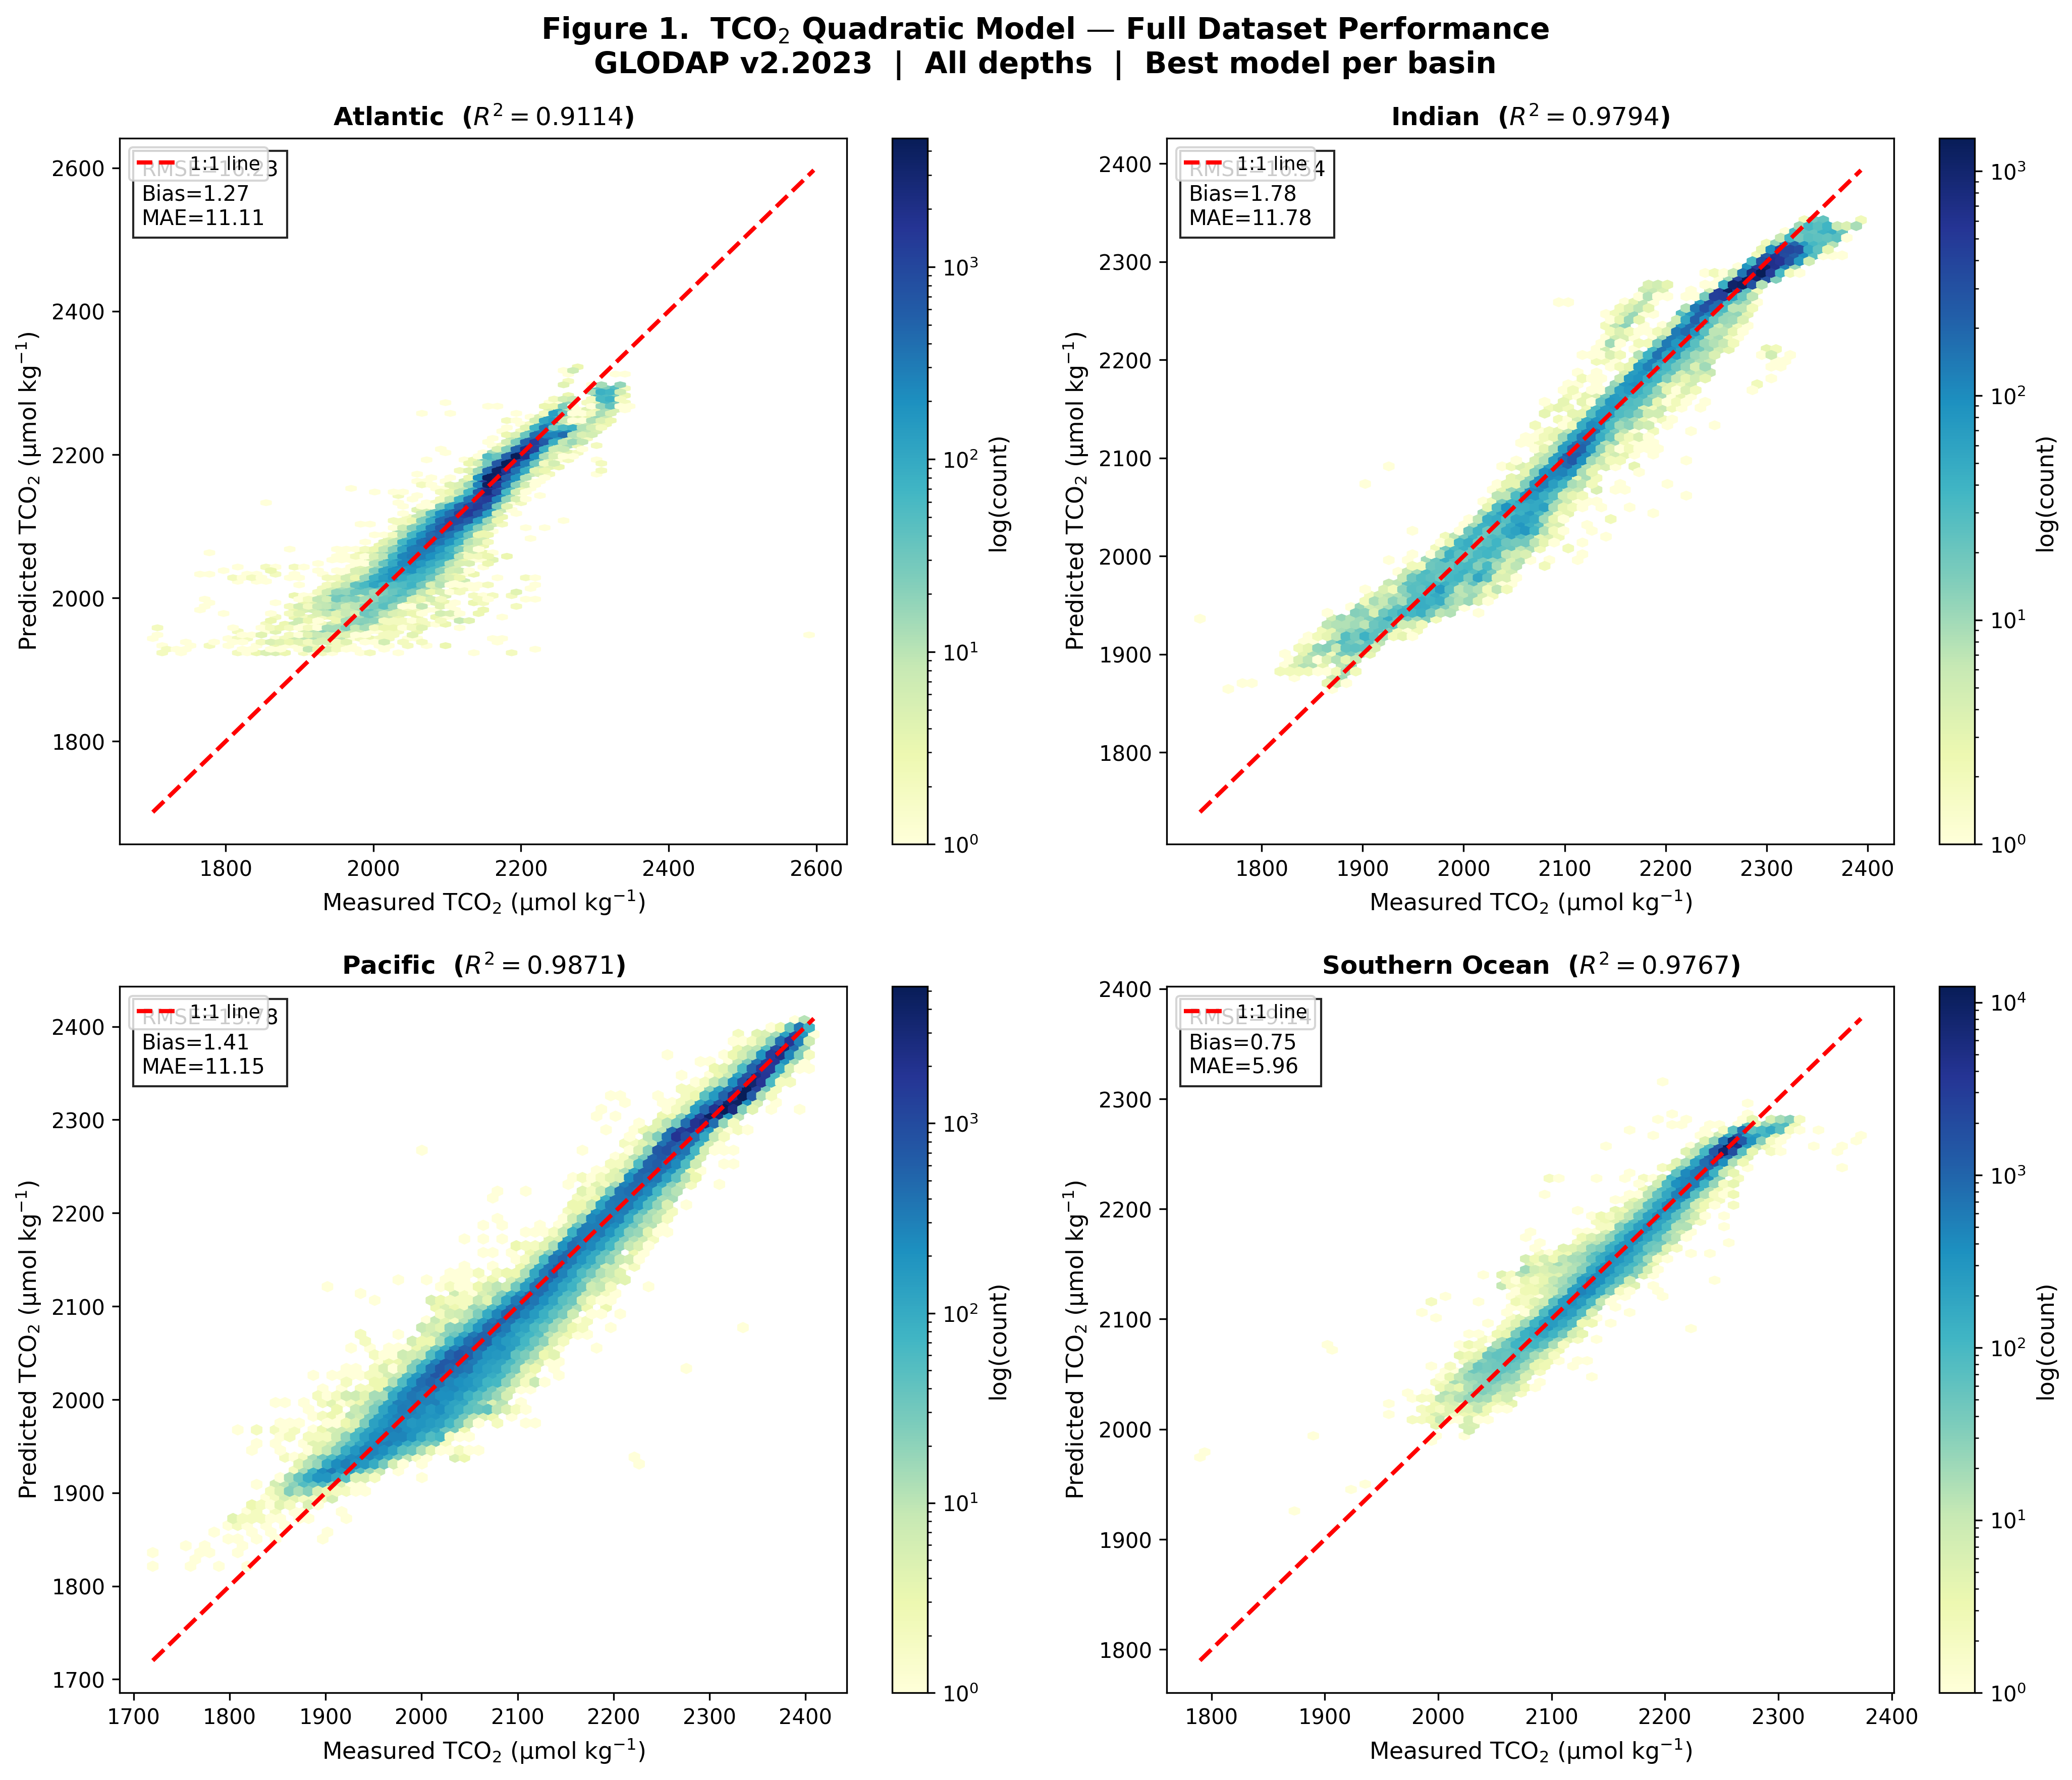
\includegraphics[width=\textwidth]{figures/final_figure1_scatter.png}
\caption{\textbf{Observed versus predicted TCO$_2$ by basin.} Hexbin density plots of observed test-set TCO$_2$ versus quadratic model predictions. The 1:1 line (red dashed) indicates perfect prediction. $R^2$, RMSE ($\mu$mol~kg$^{-1}$), and sample size are annotated. Note the different axis ranges across panels reflecting different TCO$_2$ distributions.}
\label{fig:scatter}
\end{figure}

\begin{figure}[htbp]
\centering
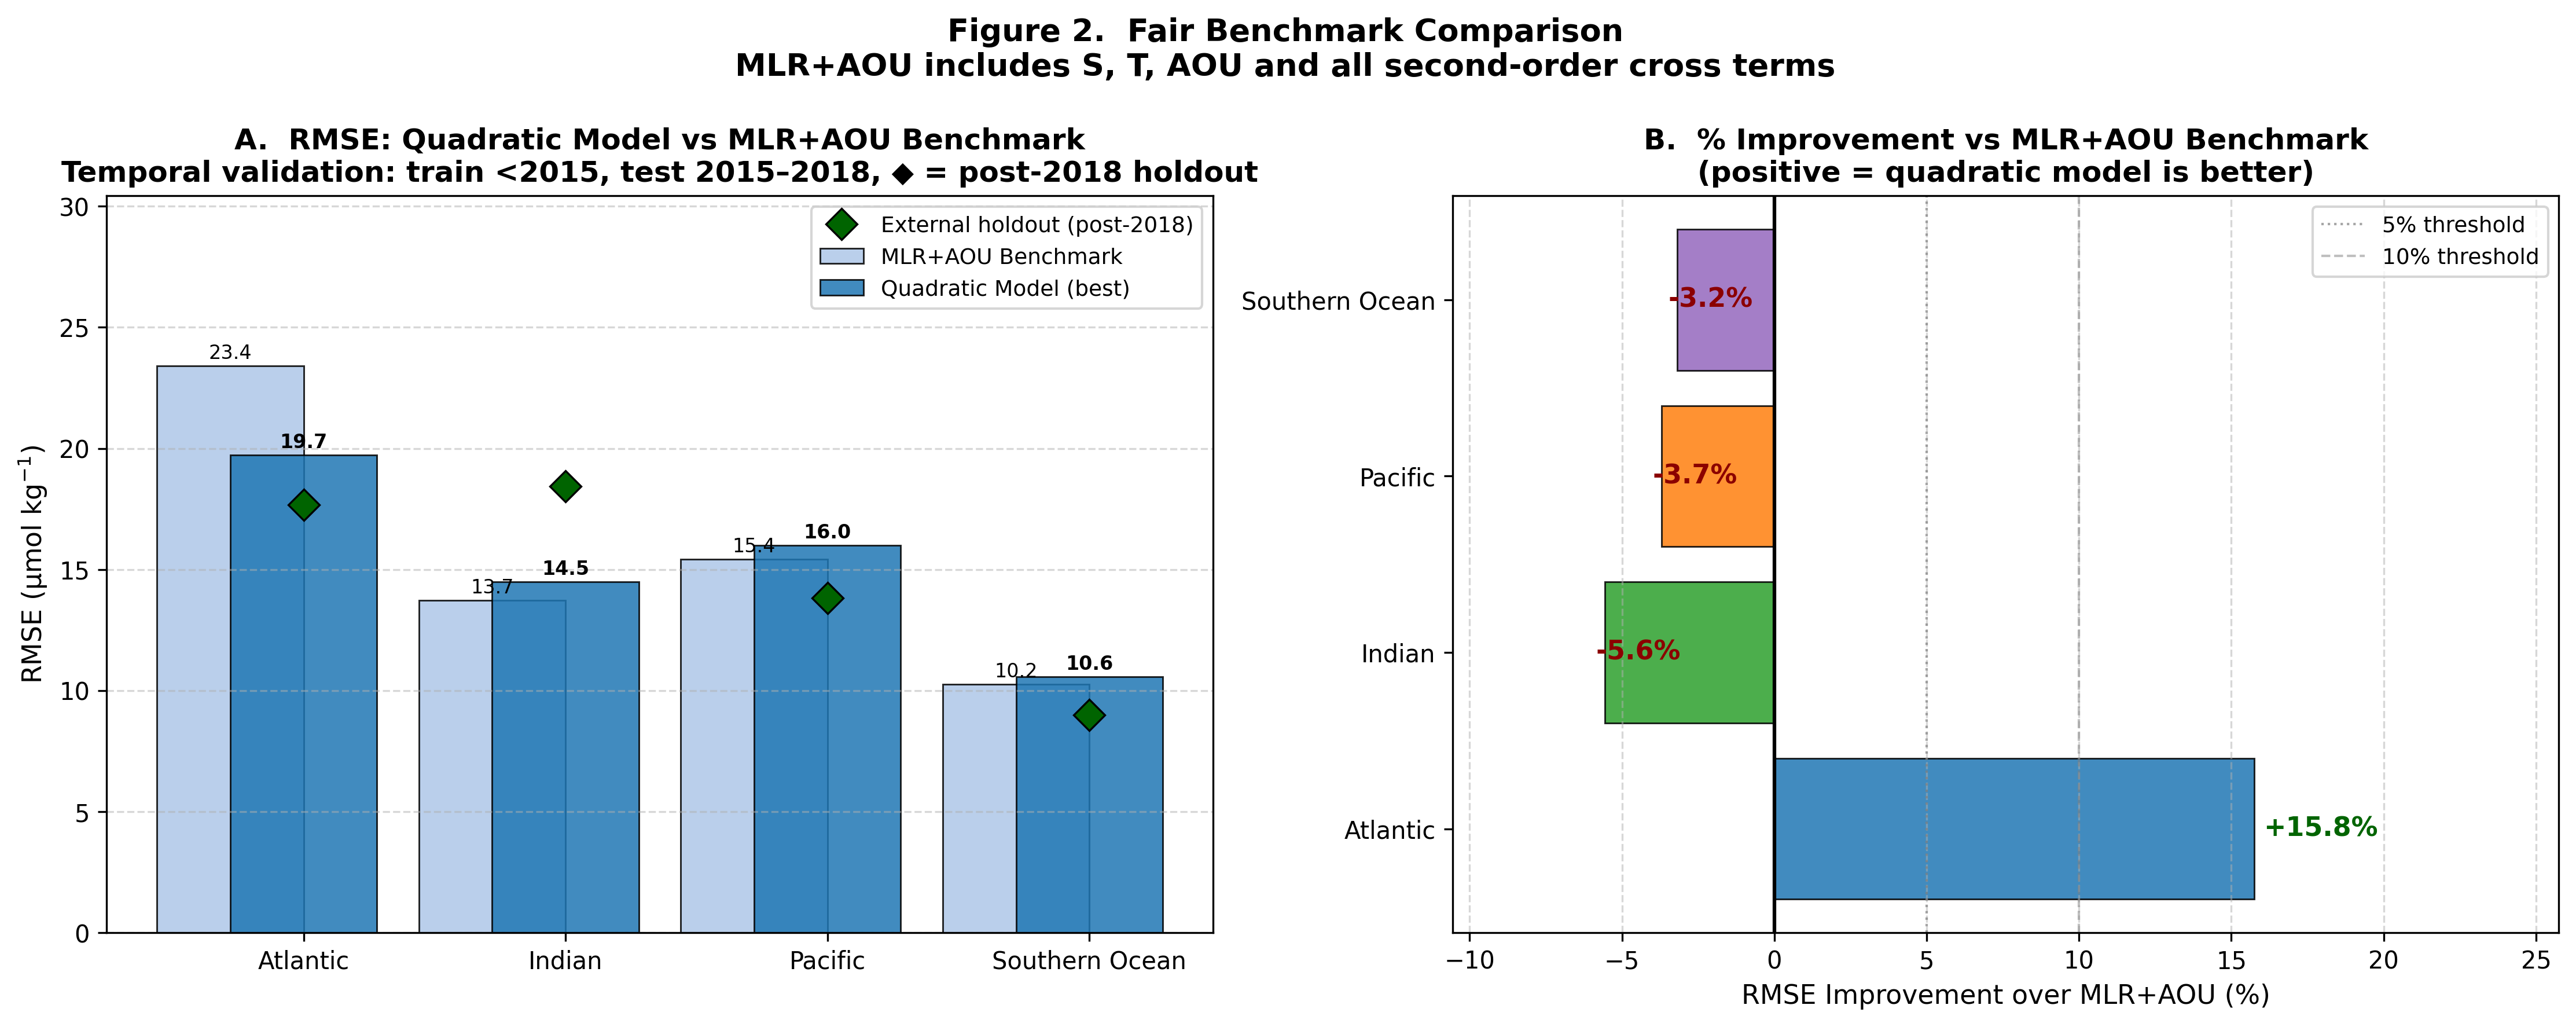
\includegraphics[width=\textwidth]{figures/final_figure2_benchmark.png}
\caption{\textbf{Benchmark comparison.} (A) RMSE by basin for the quadratic model (blue) and polynomial benchmark (light blue), with external-holdout RMSE (green diamond). (B) Percentage improvement of the quadratic model over the polynomial benchmark. Positive values indicate the quadratic model has lower RMSE.}
\label{fig:benchmark}
\end{figure}

\begin{figure}[htbp]
\centering
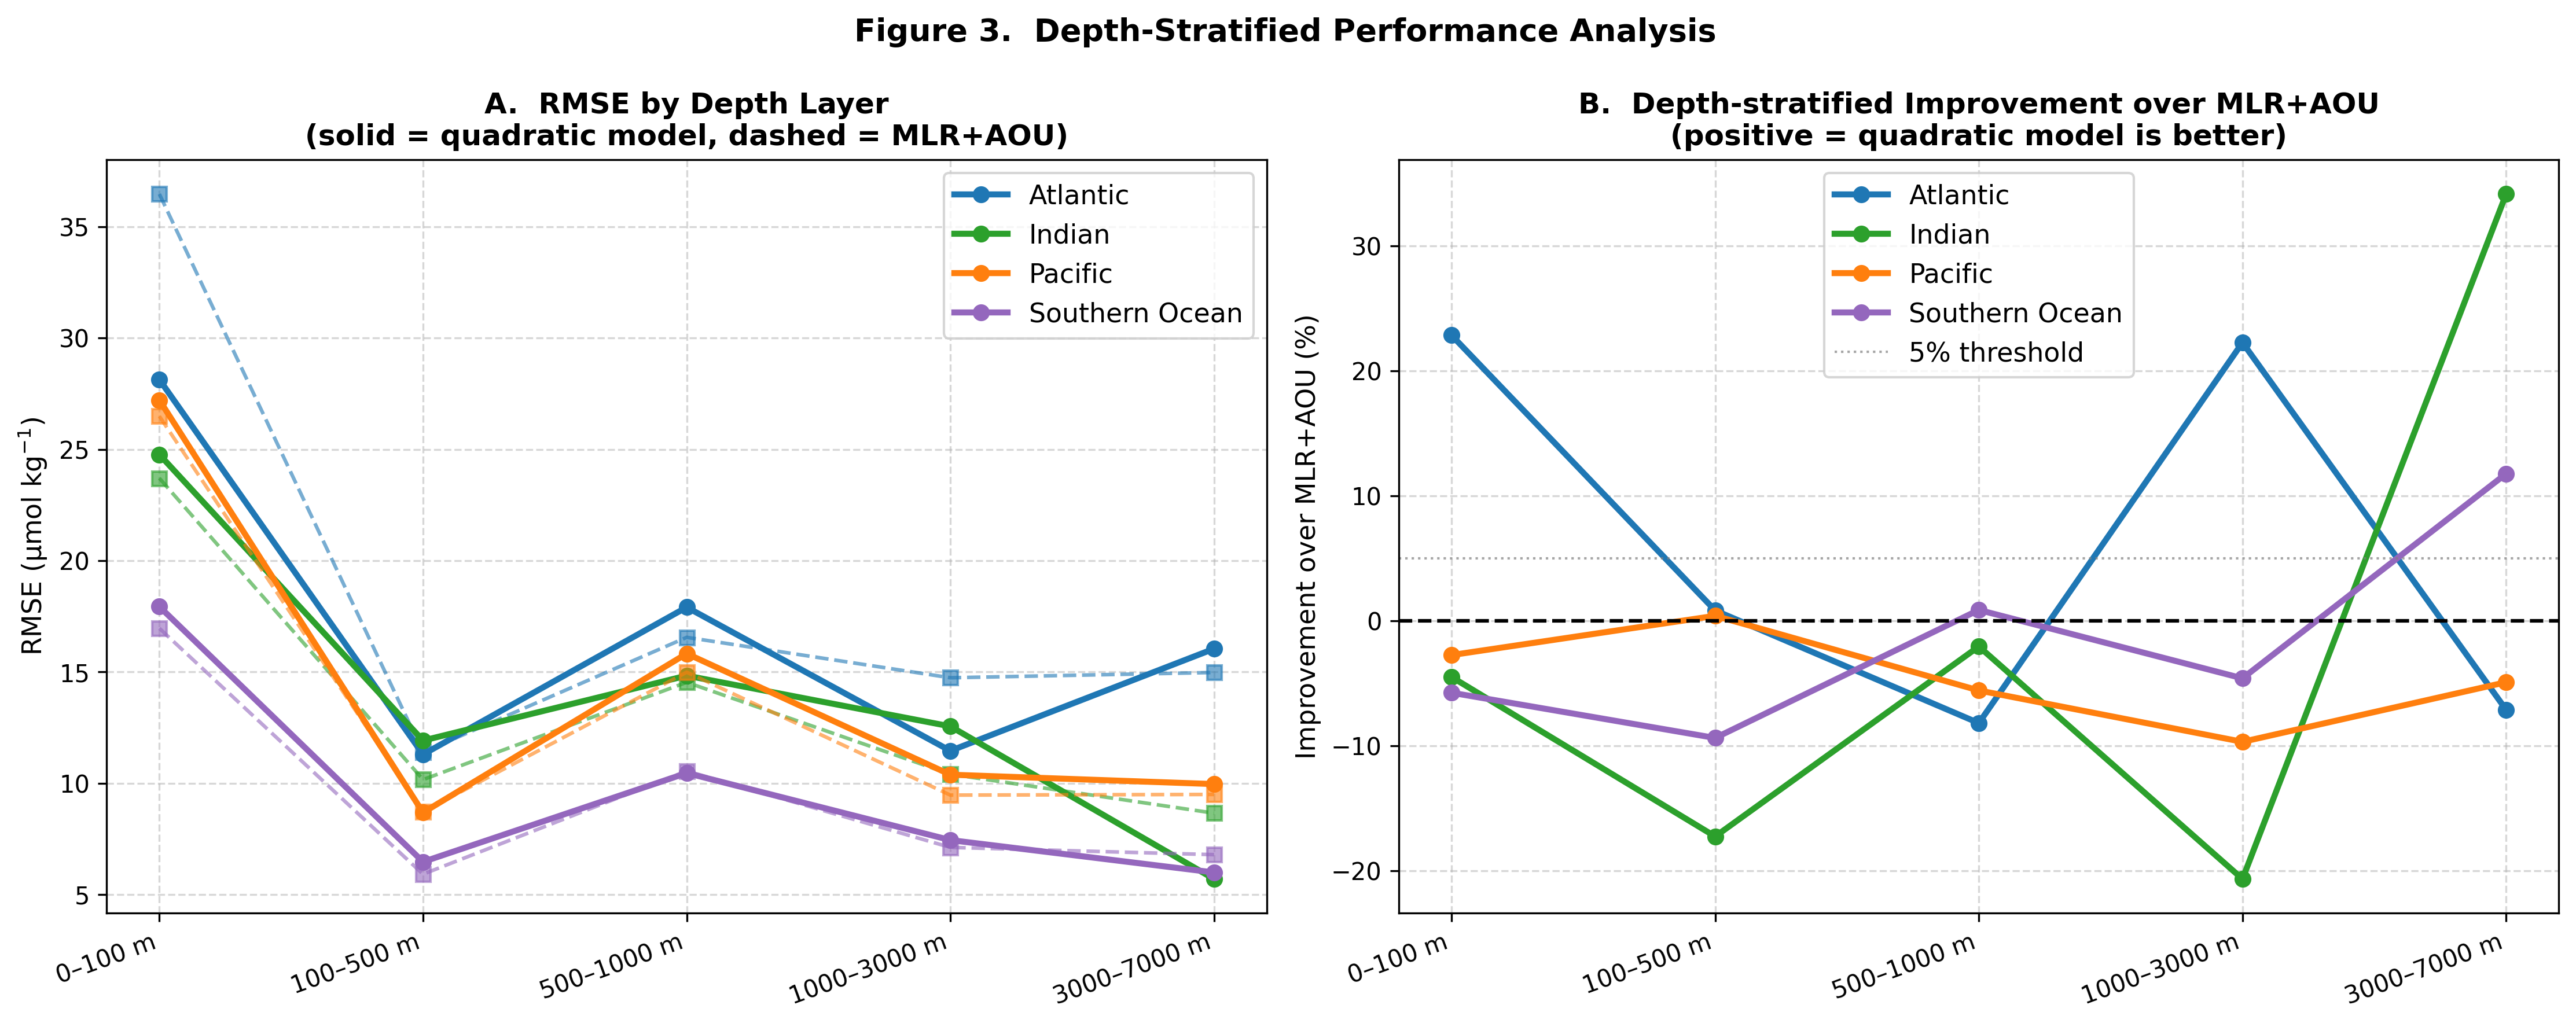
\includegraphics[width=\textwidth]{figures/final_figure3_depth.png}
\caption{\textbf{Depth-stratified performance.} (A) RMSE by depth layer for each basin (solid lines: quadratic model; dashed lines: polynomial benchmark). (B) Percentage improvement by depth. Note the strong Atlantic surface advantage (+23\%) and the Southern Ocean abyssal failure.}
\label{fig:depth}
\end{figure}

\begin{figure}[htbp]
\centering
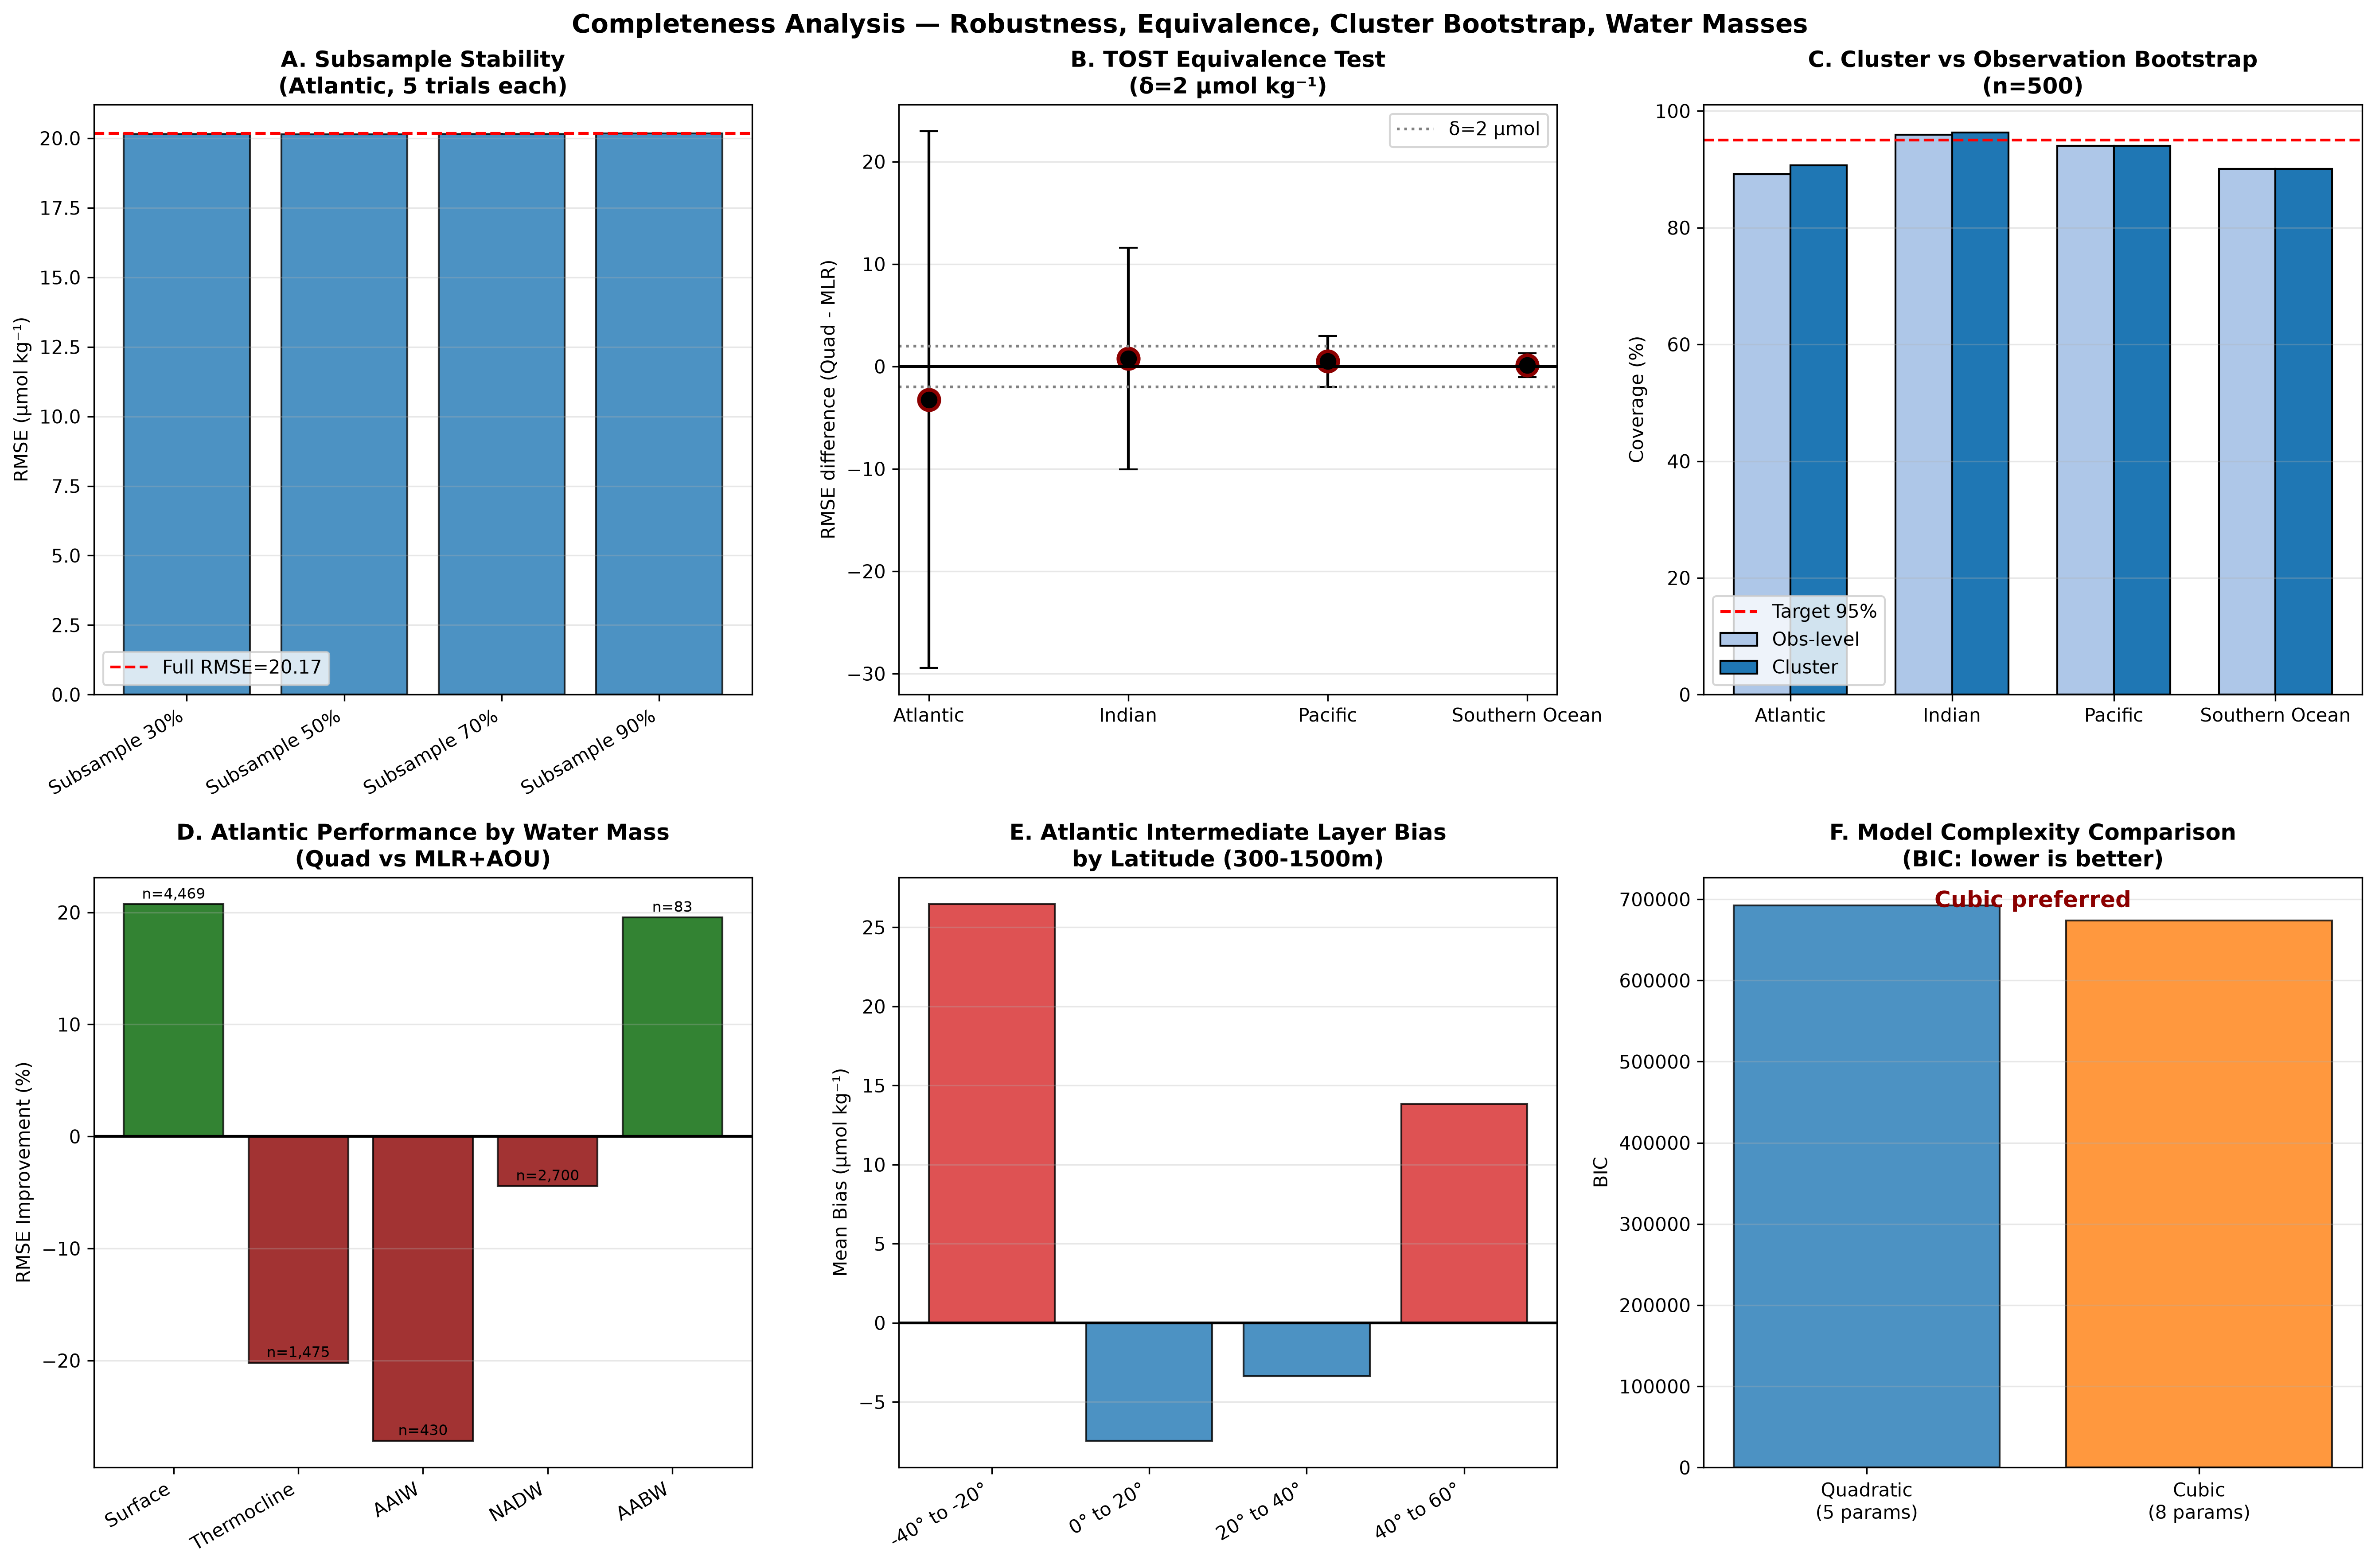
\includegraphics[width=\textwidth]{figures/COMPLETENESS_FIGURES.png}
\caption{\textbf{Robustness, equivalence, and water-mass analysis.} (A) Subsample stability. (B) TOST equivalence test confidence intervals. (C) Cluster versus observation-level bootstrap coverage. (D) Atlantic performance by water mass. (E) Atlantic intermediate-layer bias by latitude. (F) Complexity comparison (BIC).}
\label{fig:completeness}
\end{figure}

% ══════════════════════════════════════════════════════════════════════════════
% DATA & CODE
% ══════════════════════════════════════════════════════════════════════════════

\section*{Data Availability}

GLODAP v2.2023 is available at \url{https://www.glodap.info}. [Repository URL and DOI---to be added upon acceptance]

\section*{Code Availability}

[Repository URL and DOI---to be added upon acceptance. PySR configuration is documented in Table~\ref{tab:pysr_config}. Software: Python 3.14, scipy 1.18, scikit-learn 1.9, numpy 2.5, PySR version and Julia version to be documented.]

\section*{Acknowledgements}

[Funding statement---to be added]

\bibliographystyle{apalike}
\bibliography{references}

\end{document}
